\chapter{Aprendizado de máquina para séries temporais}
\label{cap:ml}

\section{O que muda quando os dados têm ordem}
Os métodos de aprendizado de máquina (florestas aleatórias, \emph{boosting}, redes neurais) foram desenhados, em sua maioria, para observações independentes. Em séries temporais, três cuidados são obrigatórios.

\subsection{Validação cruzada que respeita o tempo}
A validação cruzada aleatória (\emph{k-fold} com embaralhamento) mistura passado e futuro. Como observações vizinhas são parecidas, o modelo ``vê'' pontos quase idênticos ao que vai prever. Isso vaza informação e subestima o erro.

\begin{simulacao}[{Conferido por simulação: vazamento na validação}]
Série AR(1) muito persistente ($\phi=0{,}98$, ruído de desvio-padrão 1), floresta aleatória com 5 defasagens como variáveis explicativas. RMSE com validação cruzada aleatória: $1{,}08$. RMSE com validação temporal (treino no passado, teste no futuro): $1{,}49$. O ruído irredutível é $1{,}0$. O procedimento aleatório parece quase perfeito. O temporal mostra o desempenho real, bem pior. A diferença é puro vazamento.
\end{simulacao}

Use sempre \textbf{validação com janela móvel ou expansiva} (origem móvel, como no capítulo~\ref{cap:prev}), e, quando houver sobreposição entre janelas, deixe uma folga (\emph{gap}) entre treino e teste.

\subsection{Árvores não extrapolam}
Uma árvore (e uma floresta) prevê médias de observações já vistas. Se a série tem tendência e o futuro sai do intervalo do treino, ela fica ``presa'' no último patamar.

\begin{center}
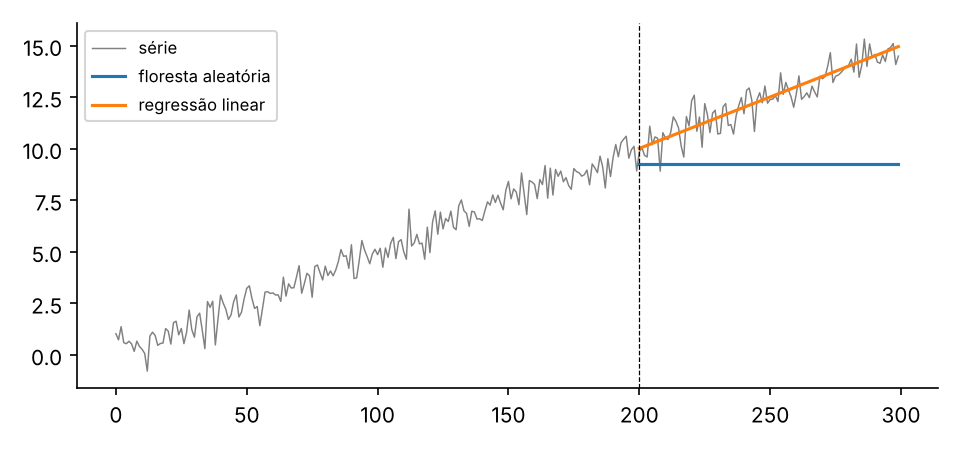
\includegraphics[width=0.75\textwidth]{fig/rf_extrapola.png}\\
\small Série com tendência linear. A floresta aleatória, treinada até $t=200$, prevê um patamar plano; a regressão linear continua a tendência.
\end{center}

\begin{simulacao}
No ponto $t=299$, a floresta previu $9{,}27$, e o valor da tendência é $14{,}95$.
\end{simulacao}

Soluções: diferenciar ou remover a tendência antes de ajustar, modelar a variação em vez do nível, ou usar um modelo híbrido (tendência linear mais floresta nos resíduos).

\subsection{Construção das variáveis explicativas}
Para transformar previsão em problema de regressão: use defasagens ($y_{t-1},\dots,y_{t-p}$), médias móveis, variáveis de calendário (mês, dia da semana, feriados) e regressores externos. Qualquer estatística construída com dados do futuro (por exemplo, normalizar com a média da série inteira) é vazamento.

\section{Duas famílias úteis}
\begin{itemize}[leftmargin=1.4em]
\item \textbf{Modelos globais}: em vez de ajustar um modelo por série, treina-se um único modelo (por exemplo, uma rede neural recorrente ou um \emph{boosting}) com milhares de séries. Ajuda quando cada série é curta ou ruidosa. É a ideia central do tutorial de Faloutsos e coautores sobre previsão em larga escala.
\item \textbf{Classificação de séries}: o problema não é prever, mas atribuir um rótulo a uma série inteira (por exemplo, normal versus anomalia num eletrocardiograma). É o foco do pacote \texttt{pyts}, que oferece técnicas como \emph{dynamic time warping}, \emph{shapelets} e representações em imagem. Não confunda com previsão.
\end{itemize}

\begin{atencao}[{Armadilhas}]
\begin{itemize}[leftmargin=1.2em]
\item \textbf{Sempre compare com o previsor ingênuo e com um ARIMA/ETS}. Muitos resultados deslumbrantes de redes profundas desaparecem diante de um \emph{benchmark} simples.
\item \textbf{Intervalos de previsão}: modelos de ML dão previsões pontuais. Para incerteza, use regressão por quantis, \emph{conformal prediction} ou simulação.
\item \textbf{Hiperparâmetros ajustados nos dados de teste}: o teste deve ser tocado uma única vez.
\end{itemize}
\end{atencao}

\begin{exercicio}
Por que embaralhar as observações antes de dividir em treino e teste é um erro numa série temporal?
\end{exercicio}
\sol{Porque faz o modelo treinar com observações do futuro e testar no passado, e porque observações adjacentes são fortemente dependentes: pontos de teste têm quase-duplicatas no treino. O erro estimado fica irrealisticamente baixo. O teste correto respeita a ordem cronológica.}
